\documentclass[10pt] {article}
%\documentclass[referee]{biom} 
%\usepackage{epsf}
%\usepackage{graphics}
%\usepackage{fullpage}
\usepackage{graphicx}
\usepackage{multirow}
\usepackage{makeidx}
\usepackage{latexsym}
\usepackage{bm}
\usepackage{amsmath}
\usepackage{amsthm}
\usepackage{amssymb}
\usepackage{setspace}

\usepackage{amssymb}
%\usepackage{lscape,rotate}
%\usepackage{rotating}
%\usepackage{xtab}
\usepackage{graphicx}
\usepackage{multirow}
\usepackage{makeidx}
\usepackage{latexsym}
\usepackage{bm}
\usepackage{amsmath}
\usepackage{amsthm}
\usepackage{amssymb}
\usepackage{setspace}
\usepackage{rotating}
%\usepackage{tabularx}
%\usepackage{booktabs}

 
\onehalfspacing
%\doublespacing
\setlength{\textheight}{22.5cm}
\setlength{\textwidth}{6.47in}
\setlength{\oddsidemargin}{-1mm}
\setlength{\topmargin}{0.1cm}
\setlength{\evensidemargin}{-5mm}
\makeindex

\newcommand{\captionfonts}{\footnotesize}
\makeatletter  
\long\def\@makecaption#1#2{
  \vskip\abovecaptionskip
  \sbox\@tempboxa{{\captionfonts #1: #2}}
  \ifdim \wd\@tempboxa >\hsize
    {\captionfonts #1: #2\par}
  \else
    \hbox to\hsize{\hfil\box\@tempboxa\hfil}
  \fi
  \vskip\belowcaptionskip}
\makeatother


\newcommand {\hide}[1] {\typeout{ #1 }}
\newcommand{\beq}{\begin{equation}}
\newcommand{\eeq}{\end{equation}}
\newcommand{\dif}[2]{\frac{{\rm d} #1}{{\rm d} #2}}
\newcommand{\ildif}[2]{{\rm d} #1/{{\rm d} #2 }}
\newcommand{\ilpdif}[2]{\partial #1/{\partial #2 }}
\newcommand{\pdif}[2]{\frac{\partial #1}{\partial #2}}
\newcommand{\pddif}[3]{\frac{\partial^2 #1}{\partial #2 \partial #3}}
\newcommand{\ilpddif}[3]{\partial^2 #1/{\partial #2 \partial #3}}
\newcommand{\comb}[2]{\left (\begin{array}{c}{#1}\\{#2}\end{array}\right )}
\newcommand{\perm}[2]{^{#1}{\rm P}_{#2}}
\newcommand{\gfrac}[2]{\mbox{$ { \textstyle{ \frac{#1}{#2} }\displaystyle}$}}
\newcommand{\defn}{\begin{quote}{\bf Definition. }}
\newcommand{\edefn}{\end{quote}}
\newcommand{\thm}{\begin{theorem}}
\newcommand{\ethm}{\end{theorem}}
\newcommand{\R}{{\sf R}}
\newcommand{\s}{{\sf S}}
\newcommand{\fnzero}{\setcounter{footnote}{0}}
\newcommand{\bmat}[1]{\left ( \begin{array}{#1}}
\newcommand{\emat}{\end{array}\right )}
\newcommand{\E}{\mathbb{E}}
\newcommand{\ts}{^{\sf T}} 
\newcommand{\its}{^{\sf -T}}
\newcommand{\fv}{\hat{\bm{\mu}}}
\newcommand{\X}{{\bf X}}
\newcommand{\Xt}{\X\ts}
\newcommand{\y}{{\bf y}}
\newcommand{\A}{{\bf A}}
\newcommand{\Qf}{{\bf Q}_{\rm f}}
\newcommand{\bp}{{\bm \beta}}
\newcommand{\rsd}{\hat {\bm \epsilon}}
\newcommand{\grad}{\nabla_\beta}
\newcommand{\tr}[1]{{\rm tr}\left ( {#1} \right )}
\theoremstyle{definition}
\newtheorem*{defin}{Definition}
\theoremstyle{plain}
\newtheorem{theorem}{Theorem}
\newcommand{\rss}{{\cal S}}
\newcommand{\eps}[3]
{{\begin{center}
\rotatebox{#1}{\scalebox{#2}{\includegraphics{#3}}}
\end{center}}
}
\newcommand{\smsz}{\small}


\begin{document}


\title{Modeling Spatiotemporal Polarization of Resident Foreign Population}

\author{Giampiero Marra, David L. Miller, and Luca Zanin
%, \\ xxxxxxxxxxxxxxxxxxxxxxx \\ E-mail: luca.zanin@studio.unibo.it 
}
%\footnote{Address for correspondence: Luca Zanin, Prometeia, via G. Marconi 43, 40122 Bologna, Italy. E-mail: luca.zanin@studio.unibo.it, tel.: +39 051 64 80 451, fax: +39 05 12 20 753.}

\maketitle


%\begin{abstract}



%\vspace{0.4cm}
%\noindent \textbf{Keywords:} 

%\noindent \textbf{JEL Classification numbers:} C14, C25, D1.

%\end{abstract}

\section{Introduction \label{IN}}

During the last decades, many scholars have shown an increasing interest in finding an explanation to the phenomenon of international migrations, as well as in monitoring the process of integration of foreigners in host countries. Several theories have been proposed, from both a macro and micro point of view, on the basis of different lines of thought. We mention, for example, the neoclassical economic theory (e.g., Borjas 1989; Massey et al. 1993), the recent assumptions of the new economics of migration (e.g., Stark and Bloom 1985; Massey et al. 1993), the aspects of dual labor market (e.g., Piore 1979; Massey et al. 1993) and the world systems theory (e.g., Wallerstein 1974; Portes and Walton 1981; Morawska 1990; Hooghe et al. 2008). In supporting international movements are also rather important migrant networks whose role is to connect migrants and non-migrants in origin and destination areas through ties of friendship, shared community origin, etc. (e.g., Massey et al. 1993). A large number of empirical cases have also been analyzed. A non-exhaustive list of examples includes the studies that have investigated the impact of foreigners on the labor market of the host country (e.g., Borjas 1994, 2003, 2005; Borjas, Freeman and katz 1996; Card 2005; Fullin and Reyneri 2010), the aspect of underemployment (Slack and Jensen 2007), the possible nexus between immigration and nation's poverty rate (Raphael and Smolensky 2009), the transmission of identities from the first to second generation immigrants (Casey and Dustmann 2010), the difference in terms of education, earnings and employment between first and second generation immigrants (Algan et al. 2010), the problems of integration of different cultures and languages (e.g., Lazer 1999; Contucci and Ghirlanda 2007), and the tendency of immigrants for living in ethnic ``enclaves'' (Edin, Fredriksson and Aslund 2003). Despite the increasing literature on international migration, to the best of our knowledge, no studies have attempted to model the spatiotemporal polarization of the incidence of resident foreigners in the total population of a country, and this is the aim of this article. The incidence is calculated as follows
\beq
\% \ incidence \ of \ resident \ foreigners_j  = \frac{number \ of \ resident \ foreigners_j}{total \ resident \ population_j} \times 100
\label{first.d1}
\eeq
where $j$ represents a specific area such municipality, province, or region (e.g., De Bartolo 2007; Lowell 2007; Coleman 2008; Miguet 2008).

In the special issue of \textit{The Economic Journal} dedicated to `the integration of immigrants and its consequences', Manning (2010) has pointed out as many European countries are experiencing a significant increase of immigrants in the population. Let us consider, for example, the Italian case. According to the official statistics of the Italian National Statistical Office (ISTAT), in the period $2003-2008$, the incidence of resident foreigners in the total population has increased from $3.4\%$ to $6.5\%$. Notice that such a growth has also been partly attributed to procedures of regularization of illegal immigrans (recall the law 189/2002; see Zincone (2002) for more details). Despite this, the speed of change in the indicator is remarkable if we consider that, on the basis of the population census (which is carried out every ten years), in the period $1991-2001$ the incidence has increased from $0.6\%$ to $2.3\%$. The recent trends of migration have been contributing to important changes from the socio-demographic and economic point of view. For example, during the last years, the official statistics have highlighted an increasing frequency in the intermarriage between Italians and foreigners, as well as in the number of entrepreneurs with foreign citizenship. For the next years, the scenario up to 2050 produced by ISTAT suggests a progressive and substantial increase of resident foreigners (about $17\%$ of the total population by 2050 as shown in Figure \ref{fig1}), a tendency that is common to many European countries (e.g., Alders, Keilman and Cruijsen 2007). Therefore, it is of paramount importance to formulate adequate social policies which can support, for instance, the integration process of immigrants in the host country. In this respect, it is crucial to promote the recognition and respect for different cultural identities with the aim of ensuring social cohesion between foreign and native people, and avoiding social unrest (e.g., Cheong et al. 2007; Van Der Veer 2003). Immigrants' rights and integration policies are typically governed by specific laws which regulate pubblic health and education services (e.g., Zincone 2006), but also professional training and the right to housing, to name a few. Several policies dedicated to foreigners also focus on offering guidance services and counseling on legal issues and administrative procedures. In this context, policy-makers can be interested in knowing whether there are areas of the country in which such policies should be strengthened as a result of a higher presence of foreigners. 

\begin{figure}[htbp]
	\centering
		\includegraphics[width=0.41\textwidth, angle=270]{Figure1.eps}
	\caption{The graphs show the trend of resident foreigners in Italy during $2003-2008$ and in forecast for the period $2009-2050$, based on the official statistics and elaborations of ISTAT. The information is reported in terms of number (divided by 1000) and incidence of resident foreigners. Both variables are calculated at the end of December of each year, except for 2001 which is obtained from the population census (October $21^{th}$). The average, low and high scenarios are by the solid and dotted lines, respectively.}
	\label{fig1}
\end{figure}

Measure (\ref{first.d1}) represents a simple well known demographic indicator for comparing different zones of a country in terms of number of foreigners every 100 resident inhabitants. The indicator returns, in this sense, an information on the type of spatial distribution of foreigners (balanced/homogeneous or unbalanced/inhomogeneous), hence identifying areas of the country with a greater or lesser presence of resident foreigners in the total population (e.g., OECD 2004). If such distribution is unbalanced in space and time, what are the factors that contribute to attract a larger number of foreigners in an area as compared to another? Inhomogeneous spatial incidence may be explained by several factors related to the characteristics of a specific area such as the presence of foreigners with the same origin (recall, for example, the network theory mentioned earlier on), and the presence of dwellings available at more favorable prices than those in other areas. Here, we focus on factors of economic and labour market nature. Specifically, we construct a composite indicator that we have named `Index of Spatial Economic Attractiveness'. It is made up of three relevant indicators, namely (i) added value per capita, (ii) unemployment rate and (iii) employment rate, and can be easily constructed for many countries given the use of standard and well known economic variables.

The empirical analysis proposed in this article addresses the issues mentioned in the previous paragraphs. Our study is carried out for Italy by using data from ISTAT which, since 2002, provides a public database with annual frequency on the number of resident foreigners at municipal level. This information is new in the panorama of Italian statistics, and currently represents the maximum spatial and temporal detail available. Spatiotemporal modelling is achieved via the use of splines which are a popular way of performing smoothing over some bounded domain $\Omega\subseteq\mathbb{R}^2$, over time (e.g., Hastie and Tibshirani 1990; Ruppert, Wand, and Carroll 2003; Wood 2006). In our context, the response (incidence of resident foreigners) is modelled as a function of its spatial coordinates and time trend. The estimated function can then be used to create smoothed maps of the geographical area of interest over time. When a geographical region has complex boundaries, as in many applied contexts, features from one part of the domain can unduly influence other parts giving rise to a phenomenon known as \textit{leakage} (e.g., Ramsay 2002). It typically occurs when a smoother inappropriately links two pats of a domain. This is problematic since it causes the fitted surface to be mis-estimated, hence leading to incorrect inference (e.g., biased incidence estimates), which is clearly not desirable. Such an issue can be overcome if the proposed spatiotemporal model can account for the structure of the domain that is under investigation. In practice, this can be achieved by using several approaches (Ramsay 2002, and references therein). Here, we construct our model by using a three-dimensional tensor product smoother combining a cubic regression spline basis function for time trend (e.g., Wood 2006) and a soap film spline basis for the spatial dimensions (Wood, Bravington and Hedley 2008).


The remainder of the article is organized as follows.


\section{Data \label{DAT}}

\subsection{The main features \label{SDC}}

The entry of foreigners from some countries of the European Union (EU) into Italy is regulated by the Schengen agreements. These allowed for the elimination of border controls, hence creating a common area of free movement among the state members (e.g., Broeders 2007). Foreigners from a non-EU country must possess a visa authorization or the necessary documents (for further details see the official website of the Ministry of the Interior http://www.interno.it). The main reasons for entering Italy as a foreigner are typically the following: study, tourism, work and family reunification. 

As pointed out by Coleman (2008), in many countries the official statistics typically report the number of resident foreign citizens, but not the number of immigrants born in foreign countries. These are not the same. Currently, the dynamics of immigration to Italy still allows the acceptance of a definition which does not distinguish between immigrants and foreign resident population identified by citizenship. This simplification is reasonable in the first phase of the immigration process in a country, and when the majority of immigrants keep their own citizenship for a long period. This is the case for Italy. Only the population census allows the best distinction between immigrants and foreigners. In this case the data can be analyzed by birthplace, citizenship at birth, and citizenship at the census time. 

Here we consider the statistics on resident foreign population. It is made up of people of non-Italian citizenship with usual residence in the country, and registered in the official population registries of the municipality in which they live. Their nationality corresponds to the country of origin, unless otherwise stated on the identity document. The Italian official statistics on resident foreign population are mainly based on administrative sources which are linked to specific laws. Since 2002, ISTAT has integrated the official statistics with a new annual public database (http://demo.istat.it). It makes available the total number of resident foreigners calculated at the end of December of each year, for each of the about 8100 municipalities. This actually represents the maximum spatial detail available. For each municipality, we have worked out measure (\ref{first.d1}) for the period $2003-2008$. As compared to the use of provincial or regional data, the municipal detail offers a better information on the spatial distribution of the foreigners in the total population.

%We think that six years can be considered a period sufficient for capturing relevant changes in spatiotemporal trends of the phenomenon under study. For istance, as shown above, the observed increase of the incidence (\ref{first.d1}) in the period 2003-2005, it was of about $100\%$. For this reason, we expect a spatiotemporal changes that can be considered significative. On the contrary, if we had observed a non-significant growth of the measure (\ref{first.d1}), we would have considered all the available period. 

As well known in demographic science, populations are dynamic over time.  The increase or decrease of foreign people, at the end of the year, is determined by the following demographic flows 
$$
RFP^{31^{th}}_{jy} = RFP^{1^{st}}_{jy} + (I_1 + I_2 + I_3+ I_4) - (D_1 + D_2 + D_3 + D_4 + AC), 
$$ 
where $RFP^{31^{th}}_{jy}$ indicates the total number of resident foreigners calculated at the end of December in the $j^{th}$ Italian municipality for the $y^{th}$ year, and $RFP^{1^{st}}_{jy}$ the number of resident foreigners at the $1^{st}$ of January. $I_{1}$ denotes people whose parents are foreigners (at least one of them being resident in the municipality), $I_{2}$ the foreign citizens who asked to transfer their residence from an Italian municipality to the current one, $I_{3}$ those who asked to transfer their residence from abroad, and $I_{4}$ refers to recording operations due to several reasons. $D_{1}$ represents the resident foreigners who died during the year, $D_{2}$ those removed from the registry of the current municipality because transferred to another one, $D_{3}$ foreigners removed from the registry because transferred their residence abroad, $D_{4}$ refers to cancellations, and \textit{AC} denotes the resident foreigners who obtained the Italian citizenship during the year. 

Acquisition of the Italian citizenship by foreigners is regulated by law 91 of the $5^{th}$ of February 1992 and subsequent amendments and additions. Foreigners can acquire the Italian citizenship mainly for marriage with an Italian or for `naturalization'. The last case refers to a situation in which the foreigner has lived in the country from a certain period of time. Such a period may vary based on the following criteria: (a) at least 10 years for non-EU citizens, (b) at least 4 years for EU citizens, (c) at least 5 years for political refugees or stateless persons, and (d) at least 5 years for adult individuals who been adopted by Italian citizens. These do not provide a list of all possible cases. Moreover there exist further cases to obtain the citizenship. See http://www.interno.it for more details. 

Once the foreigners have acquired the Italian citizenship, they are included in the Italian population's statistics. Currently, no information on the number of resident Italian citizens by origin is available. It could be interesting to know the number of people that are Italian by birth, and those who obtained the citizenship. For instance, this information could be useful for monitoring the ethnic and cultural diversity in the population. However, the multi-ethnic or multi-cultural aspect is not of interest given our purposes. %, but could be useful for a possible extension of this work. 

The phenomenon of illegal foreigners (e.g., Carter 1999; Hillman and Weiss 1999; De Bartolo 2007; Bchir 2008; Cangiano 2008) and its respective quantification (e.g., Strozza 2004) is also important to policy-makers and scholars. It refers to foreigner people who are not in possession of a visa authorization, the necessary documents or a valid permission to be in the country. In the literature, several solutions have been proposed in order to quantify this phenomenon, but all of them are subject to criticism especially related to the magnitude of the error in the estimates. For this reason, we only make use of the official data on the resident foreign population, hence avoiding the introduction of possible distorting factors which are not directly controllable and quantifiable. %The assumptions made in our study is that the incidence of foreigners (\ref{first.d1}) can be very close to the real data observed in hypotesis of absence of illegal foreigners in the country.


\subsection{The demographic contribution of the foreign population \label{DEM}}

Assuming the absence of migration flows from abroad in predicting the population until 2052 for each of the 27 European countries, Bijak et al. (2007) showed that many nations could register a declines of the population resident. The main causes are the progressive aging of the population structure and to the low fertility rate. In particular, for Italy they have estimated a possible decrease of the population from 57 million of 2002 to about 43 million for 2052. The ratio between the population with more than 64 years and young population (0-14 years) was equal to 143.4 at the end of 2008 (index equal to 156.2, considering only the population with Italian citizenship). This means that the elderly population is about 43 percent more than the young population. The index computed only considering the resident foreign population is equal to 11.2 (we point out that the average age of the foreigners resident is of about 30 years). Looking to the most recent fertility rate released by ISTAT, the average number of children for each Italian women in childbearing age (from 15 to 49 years) is equal to 1.33; a number much low if compared with the average of 2.05 children for the foreign women. The total fertility rate considering both italian and foreign womens is equal to 1.41. 
Coleman (2008) recalls that ``typically, in low-mortality populations a total fertility of about 2.04 is regarded as the `replacement level', that is, a level sufficient to replace the population in the long-run, ignoring migration''. However, according with other scholars, Coleman has also pointed out that given the impact of foreigners in the population structure of many countries, the measure of total fertility, and hence the level of replacement, must taken into account also the contribution of immigrants. In recent years, the foreign presence in Italy has contributed not only to population growth, but also to the reduction of the aging index and to the improvement of the total fertility rate. 
The profile of the nationalities of the foreigners resident in Italy is evolving. In 2003, the ranking of the top three countries of immigration  was represented from Albania ($13.6\%$), Morocco ($12.7\%$) and Romania ($8.9\%$). In 2008, Romania was the first country represented ($20.5\%$), followed by Albania ($11.3\%$) and Morocco ($10.4\%$). The significant increase of the Romanian population in Italy has occured with the country's entry in the European Union ($1^{th}$ January 2007). They are the predominant nationality in 14 regions out of 20. Ban (2009) has pointed out that Italy hosts the largest Romanian community outside Romania and almost half of the entire Romanian migrant stock. The choice of Italy by Romanian population can be explained by the presence of Italian small companies, the economic links in Romania, the accessible language for this population, and so on. As an overview, in 2008 the foreign population resident in Italy was for $53.6\%$ of European origin, $22.4\%$ African, $15.8\%$ Asian,  $8.1\%$ American, and a marginal share from Oceania ($0.1\%$).


\section{Methodology \label{METH}}

\subsection{Model specification \label{MS}}

The model we employ belongs to the class of generalized additive models (GAMs, Hastie and Tibshirani 1990). They allow for  complex relationships between covariates and response variable, which are crucial to uncover interesting features in the data. Notice that the incidence of resident foreigners exhibits a positively skewed distribution. For this reason, a gamma distribution provides a realistic description of the response variable. The proposed model is as follows
\beq
\text{log}\left\{\E(\texttt{inc.rf}_{it})\right\} = f(\texttt{year}_t,\texttt{n}_i,\texttt{e}_i), \quad \texttt{inc.rf}_{it} \sim \text{Gamma},          
\label{PropM}
\eeq
for $i=1,\ldots,8094$ and $t=1,\ldots,6$. The log link function ensures positive fitted values. $\texttt{inc.rf}_{it}$, $\texttt{n}_i$, and $\texttt{e}_i$ represent the variables percentage incidence of resident foreigners, northing, and easting, respectively. The function $f$ is a multidimensional smooth of \texttt{year}, \texttt{n}, and \texttt{e} which models the joint effect of these variables on \texttt{inc.rf}. Notice that we want both the space and time dimension to have an optimal degree of smoothness in terms of the bias variance trade-off. This means that the chosen smoother has to be invariant to the relative scaling of space (km) and time (years). This can be achieved by using a multidimensional tensor product smooth combining a cubic regression spline basis for time trend and an \textit{isotropic} soap film spline basis for the two spatial dimensions \texttt{n} and \texttt{e}, since the smoother should not depend on the coordinate system used and account for the structure of the geographical domain under investigation (details are given in the next two sections). The smooth component in (\ref{PropM}) is subject to identifiability constraints; see Wood (2006) for more details.

\subsection{A three-dimensional tensor product smoother for time and space \label{3D}}

The construction of a three-dimensional scale invariant tensor product smoother of time and space is based on a marginal one-dimensional spline basis for time and a two-dimensional marginal smooth for space, with associated quadratic penalties measuring their roughness. We omit the subscripts $i$ and $t$ for simplicity. Let us assume that we have two low-rank regression spline bases of any type to represent the smooth functions $f_\text{year}$ and $f_\text{space}$, we can write (e.g., Ruppert, Wand and Carroll 2003)
$$
f_\text{year}(\texttt{year})=\sum_{l=1}^L \alpha_l a_l(\texttt{year})=\textbf{X}_\text{year}\bm\alpha \ \ \text{and} \ \ f_\text{space}(\texttt{n},\texttt{e})=\sum_{r=1}^R \gamma_r d_r(\texttt{n},\texttt{e})=\textbf{X}_\text{space}\bm\gamma,
$$
where the $a_l(\texttt{year})$ and $d_r(\texttt{n},\texttt{e})$ are known cubic regression spline and soap film basis functions, with corresponding parameters $\alpha_l$ and $\gamma_r$, $L$ and $R$ are the spline dimensions of the two smooth components, and $\textbf{X}_\text{year}$ and $\textbf{X}_\text{space}$ are marginal model matrices evaluating the basis functions with parameter vectors $\bm\alpha$ and $\bm\gamma$ (Wood 2006, 2008). In order to set up a three-dimensional tensor product smoother for time and space we need $f_\text{year}(\texttt{year})$ to vary smoothly within the space dimensions. This can be achieved by allowing the parameters $\alpha_l$ to vary smoothly with \texttt{n} and \texttt{e}. Using the spline set-up for $f_\text{space}(\texttt{n},\texttt{e})$ we can write (e.g., Wood 2006)
$$
\alpha_l(\texttt{n},\texttt{e})=\sum_{r=1}^R \gamma_{lr} d_r(\texttt{n},\texttt{e})
$$    
which results in
$$
f(\texttt{year},\texttt{n},\texttt{e})=\sum_{l=1}^L \sum_{r=1}^R \gamma_{lr} d_r(\texttt{n},\texttt{e}) a_l(\texttt{year}). 
$$
For any particular set of observations of \texttt{year}, \texttt{n}, and \texttt{e}, there exists a simple relationship between the matrix $\textbf{X}$ evaluating the tensor product smooth at these observations, and the model matrices $\textbf{X}_\text{year}$ and $\textbf{X}_\text{space}$ evaluating the marginal smooths at the same observations. Ordering appropriately the parameters $\gamma_{lr}$ into a vector $\bm\theta$, the $i^{th}$ row of $\textbf{X}$ is given by $\textbf{X}_{i}=\textbf{X}_\text{year,i}\otimes\textbf{X}_\text{space,i}$, where $\otimes$ is the Kronecker product. 

Within the GAM context, it is necessary to quantify the roughness of the smooth functions in the model so that over-fitting can be accounted for and hence avoided during the parameter estimation process (e.g., Marra and Radice 2010). As for the penalty associated with this tensor product basis, it is possible to start from roughness measures associated with the marginal smooths $f_\text{year}(\texttt{year})$ and $f_\text{space}(\texttt{n},\texttt{e})$. Suppose that functionals $Js$ measuring the roughness of the smooth terms are available, and that these can be written as quadratic forms in the marginal parameters, we have that
$$
J_\text{year}(f_\text{year})=\bm\alpha\ts\textbf{S}_\text{year}\bm\alpha \ \ \text{and} \ \ J_\text{space}(f_\text{space})=\bm\gamma\ts\textbf{S}_\text{space}\bm\gamma,
$$
where the $\textbf{S}$ matrices contain known coefficients whose values depend on the chosen bases for time and space. For instance, the second-order cubic spline penalty for $f_\text{year}(\texttt{year})$ evaluates $J_\text{year}(f_\text{year})=\int\left( \partial^2 f_\text{year}/\partial year^2 \right)^2 dyear$, but it may be more complex (e.g., Wood 2006, 2008). Following, for example, Zanin and Marra (2010), an overall penalty for the tensor product smooth can be obtained by applying the penalties of $f_\text{space}(\texttt{n},\texttt{e})$ to the varying coefficients of the marginal smooth $f_\text{year}(\texttt{year})$, $\alpha_l(\texttt{n},\texttt{e})$,
$$
\sum_{l=1}^L J_\text{space}\left\{  \alpha_l(\texttt{n},\texttt{e}) \right\},
$$ 
and the penalties of $f_\text{year}(\texttt{year})$ to the varying coefficients of the marginal smooth $f_\text{space}(\texttt{n},\texttt{e})$, $\gamma_r(\texttt{year})$,  
$$
\sum_{r=1}^R J_\text{year}\left\{  \gamma_r(\texttt{year}) \right\}.
$$ 
It follows that the roughness penalty of $f(\texttt{year},\texttt{n},\texttt{e})$ can be measured as 
$$
J(f)=\lambda_\text{space} \sum_{l=1}^L J_\text{space}\left\{  \alpha_l(\texttt{n},\texttt{e}) \right\} + \lambda_\text{year} \sum_{r=1}^R J_\text{year}\left\{  \gamma_r(\texttt{year}) \right\},
$$
which can also be written as
$$
\lambda_\text{space} \bm\theta\ts \textbf{I}_L \otimes \textbf{S}_\text{space} \bm\theta + \lambda_\text{year} \bm\theta\ts \textbf{S}_\text{year} \otimes \textbf{I}_R  \bm\theta,
$$
where, once again, the vector $\bm\theta$ contains the tensor product smooth parameters. The $\lambda$ are smoothing parameters controlling the trade-off between model fit and model smoothness. The next section shows how $f_\text{space}$ and $\textbf{S}_\text{space}$ can be constructed.   


\subsubsection{Soap film \label{SF}}

As alluded to above, the smoother used for the spatial part of the model must take into account of the fact that the borders of Italy, Sicily and Sardinia represent both physical and administrative geographic features. Clearly a rather na�ve model would smooth over the bounding box encompassing all of the region we wish to draw inference on, this is not useful; first, because there are no immigrants in the sea (at best there are merely potential immigrants) and second, because smoothing over this whole area would cause leakage, as mentioned previously.



Leakage occurs when a smoother inappropriately links two pats of a domain, this can happen when a two peninsulae jut out into the sea with different population densities on either side. Say one has a very high density, where as the other is significantly lower. Most smoothers will not respect that the two areas are different and should be treated so. Rather, the model will ``smooth across'' this gap, causing the high functional values to ``leak'' into the low valued peninsula and vice versa. 

There are, of course, situations in which leakage is appropriate. For example, in a study of the propagation of a chemical through a river system, there are several mechanisms to transport the chemical (eg. surface water flow, animals) other than the river itself. Therefore there must be a motivation for why we wish to use a model that specifically prevents leakage. This is the case here, as there is no particular reason we should believe that immigration should be continuous across physical boundaries such as the Mediterranean Sea.


THOUGHT: Might be worth including a Ramsay horseshoe if we're going to make a big deal of leakage?


The soap film smoother (\cite{soap}) uses a rather simple physical model to prevent leakage from occurring. First, consider the domain boundary to be made of wire, then dip this wire into a bucket of soapy water, you will then have (provided it doesn't pop(!)) a soap film in the same of your boundary. Now consider the wire to lie in the $x-y$ plane and the height of the soap film at a given point to be the functional value of the model. This film is then distorted smoothly by moving it toward the data, while minimising the surface tension in the film. The domain ($\Omega$) is bounded by some polygon with boundary conditions estimated by a cyclic spline.

Mathematically, the soap film smoother is constructed by first specifying a set of functions $\rho_k(x,y)$, which are each solutions to the Laplace equation in two dimensions:
\beq
\frac{\partial^2\rho}{\partial x^2} + \frac{\partial^2\rho}{\partial y^2} = 0
\eeq
except at one of the knots ($x^*_k,y^*_k$). Then, solving Poisson's equation in 2-dimensions:
\beq
\frac{\partial^2 g_k}{\partial x^2} + \frac{\partial^2 g_k}{\partial y^2} = \rho
\label{soap-poisson}
\eeq
with $\rho=\rho_k(x,y)$, where $k$ indexes the knots, the set of basis functions for the soap film smoother, $g_k(x,y)$ is found, along with $a(x,y)$ (the solutions to (\ref{soap-poisson}) when $\rho=0$). These bases are then summed to form:
\beq
f(x,y)=a(x,y)+\sum_{k=1}^n \gamma_k g_k(x,y),
\eeq
the soap film smoother, where the $\gamma_k$ are parameters to be estimated. The (isotropic) penalty term is:
\beq
\int_\Omega \Big(\frac{\partial^2 f}{\partial x^2}+\frac{\partial^2 f}{\partial y^2} \Big)^2\text{d}x\text{d}y,
\eeq
This differs from the standard thin plate regression spline penalty since: (\emph{i}) the integration occurs only over $\Omega$, (\emph{ii}) there is no mixed derivative term, and (\emph{iii}) the whole integrand is squared rather than each term individually. This allows the $x$ and $y$ term's derivatives to be traded off against each other so the nullspace of the penalty is infinite dimensional. This allows those functions in the nullspace to be sufficiently wiggly to meet any boundary conditions.

THOUGHT: Take some time to say how shit Kriging is? :)



PROBABLY DON'T NEED THIS:
The solution of the PDEs above, yielding the basis and penalty, is the most computationally expensive part of the procedure. Knots to use for $x_k^*$ and $y_k^*$ must be specified, usually using a grid. Numerical problems occur when knots are placed in boundary cells in the PDE solution grid.


Although mathematically elegant, the soap film smoother is a rather complex model. It also treats the boundary as a special case and uses a cyclic spline in order to approximate the boundary values. This treatment of the boundary seems rather unnatural and it may not always be physically realistic to consider the boundary in such a way.

-------------------------------------------------------------------------------------------------------------------------


As alluded to above, the smoother used for the spatial part of the model must take into account of the fact that the borders of Italy, Sicily and Sardinia represent both physical and administrative geographic features. Clearly a rather na\"ive model would smooth over the bounding box encompassing all of the region we wish to draw inference on, this is not useful; first, because there are no immigrants in the sea (at best there are merely potential immigrants) and second, because smoothing over this whole area would cause leakage, as mentioned previously.

Leakage occurs when a smoother inappropriately links two pats of a domain, this can happen when a two peninsulae jut out into the sea with different population densities on either side. Say one has a very high density, where as the other is significantly lower. Most smoothers will not respect that the two areas are different and should be treated so. Rather, the model will ``smooth across'' this gap, causing the high functional values to ``leak'' into the low valued peninsula and vice versa.

There are, of course, situations in which leakage is appropriate. For example, in a study of the propagation of a chemical through a river system, there are several mechanisms to transport the chemical (eg. surface water flow, animals) other than the river itself. Therefore there must be a motivation for why we wish to use a model that specifically prevents leakage. This is the case here, as there is no particular reason we should believe that immigration should be continuous across physical boundaries such as the Mediterranean Sea.

The soap film smoother (CITE: Wood et al) uses a rather simple physical model to prevent leakage from occurring. First, consider the domain boundary to be made of wire, then dip this wire into a bucket of soapy water, you will then have a soap film in the same shape as the boundary (provided it doesn't pop(!)). Now consider the wire to lie in the $\texttt{n}$-$\texttt{e}$ plane and the height of the soap film at a given point to be the functional value of the model. This film is then distorted smoothly by moving it vertically toward the data, while minimising the surface tension in the film. The domain ($\Omega$) is bounded by some polygon ($B$) which, in this case is the coastlines. The boundary conditions on $B$ are estimated using a cyclic spline (CITE Simon book, p 151).

Mathematically, the soap film smoother is constructed by first specifying a set of functions $\rho_k(\texttt{n},\texttt{e})$, which are each solutions to the Laplace equation in two dimensions:
\beq
\frac{\partial^2\rho}{\partial \texttt{n}^2} + \frac{\partial^2\rho}{\partial \texttt{e}^2} = 0
\eeq
except at one of the knots ($\texttt{n}^*_k,\texttt{e}^*_k$). Then, solving Poisson's equation in 2-dimensions:
\beq
\frac{\partial^2 g_k}{\partial \texttt{n}^2} + \frac{\partial^2 g_k}{\partial \texttt{e}^2} = \rho
\label{soap-poisson}
\eeq
with $\rho=\rho_k(\texttt{n},\texttt{e})$, for $k$ indexing the knots. When the boundary condition $\rho=0$ is applied, the set of basis functions for the soap film smoother, $g_k(\texttt{n},\texttt{e})$ is found. 

A `boundary function', $f_\text{bnd}(r)$, modelled using cyclic splines (as in CITE Simon book p151) will have the form
\beq
f_\text{bnd}(r)=\sum_{j=1}^J \alpha_j \delta_j(r),
\label{soap-cyclic}
\eeq
where $r$ is the distance along the boundary, the $\alpha$ are the parameters to be estimated and $\delta_j$ are known basis functions. To ensure that the spline is cyclic the usual constraint is enforced: that the value of the function at the first knot is the same as that at the last knot up to their second derivatives. The parameters, $\alpha_j$, are then used to for the parameters in the basis function representation of the boundary-condition-induced function $a(\texttt{n},\texttt{e})$. This can be shown to have the form:
\beq
a(\texttt{n},\texttt{e})=\sum_{j=1}^J \alpha_j a_j(\texttt{n},\texttt{e}),
\eeq
where the functions, $a_j(\texttt{n},\texttt{e})$, can be found by solving (\ref{soap-poisson}) with $\rho(\texttt{n},\texttt{e})\equiv 0$ with the boundary condition resulting from setting $\alpha_j=1$ (and all other $\alpha_i$ to zero) in (\ref{soap-cyclic}), using the same methods as for the $g_k(\texttt{n},\texttt{e})$, above.

These bases are then summed to form:
\beq
f_\text{int}(\texttt{n},\texttt{e})=a(\texttt{n},\texttt{e})+\sum_{k=1}^n \gamma_k g_k(\texttt{n},\texttt{e}),
\eeq
the soap film smoother for the interior, where the $\gamma_k$ are parameters to be estimated. One can think of $a(\texttt{n},\texttt{e})$ as an offset dictated by the estimated boundary conditions on $\Gamma$ and the sum of the $g_k(x.y)$ as the smooth to the data inside $\Gamma$.


The penalty is split into two parts, one for the cyclic smooth around the boundary and one for the internal smooth. Writing $\bm\beta$ as the vector of all smooth coefficients for the soap film, $\bm\gamma$ for the boundary smooth parameters and $\bm\alpha$ for the interior, we have:
\beq
\bm\beta^\text{T}S_\text{space}\bm{\beta} = \lambda_\text{bnd} \bm\gamma^\text{T}S_\text{bnd}\bm{\gamma} + \lambda_\text{int} \bm{\alpha}^\text{T}S_\text{int}\bm{\alpha},
\eeq
where $S_\text{space}$ is the total penalty for the spatial part of the smooth, $S_\text{int}$ is the interior penalty and $S_\text{bnd}$ is the cyclic spline boundary penalty. The $\lambda$ are the smoothing parameters for the boundary and interior smooths respectively. We now look at the two parts of the penalty individually.

The isotropic interior penalty term is calculated as:
\beq
S_\text{int} = \int_\Omega \Big(\frac{\partial^2 f_\text{int}}{\partial \texttt{n}^2}+\frac{\partial^2 f_\text{int}}{\partial \texttt{e}^2} 
\Big)^2\text{d}\texttt{n}\text{d}\texttt{e},
\eeq
Differing from the standard thin plate regression spline penalty since: (\emph{i}) the integration occurs only over $\Omega$, (\emph{ii}) there is no mixed derivative term, and (\emph{iii}) the whole integrand is squared rather than each term individually. This allows the $\texttt{n}$ and $\texttt{e}$ term's derivatives to be traded off against each other so the nullspace of the penalty is infinite dimensional. This allows those functions in the nullspace to be sufficiently wiggly to meet any boundary conditions.

The penalty for the cyclic spline running about the boundary is calculated as:
\beq
S_\text{bnd} = \int_B \frac{\partial^2 f_\text{bnd}}{\partial r^2} \text{d}r, 
\eeq
as normal.

The solution of the PDEs above, yielding the basis and penalty, is the most computationally expensive part of the procedure. Knots to use for $\texttt{n}_k^*$ and $\texttt{e}_k^*$ must be specified, here we use a grid. Further detail on this is given below.






\subsection{Parameter estimation \label{PE}}

In model (\ref{PropM}), replacing $f$ with its tensor product expression yields a generalized linear model (McCullagh and Nelder, 1989) whose design matrix contains the spline bases representing the smooth component in the model. This means that in principle such
a model can simply be estimated by maximum likelihood (ML). However, in a smoothing spline context, unpenalized parameter estimation is likely to result in smooth component estimates that are too `wiggly', hence undermining the utility of such a model. This can be overcome by penalized ML, where the use of penalties allows for the suppression of that part of smooth term complexity which has no support from the data (e.g., Marra and Radice 2010). Specifically, the model can be fitted by minimization of
\beq
D(\bm\theta) + \bm\theta\ts\textbf{S}\bm\theta \ \  \text{w.r.t.} \ \  \bm\theta.
\label{Dev}
\eeq
The model deviance, $D$, is defined as $2\phi(l_{\text{sat}}-l)$, where $\phi$ is a dispersion parameter, $l$ is the log-likelihood of the model and $l_{\text{sat}}$ the maximum value for the log-likelihood of the model with one parameter per datum. $\textbf{S}=\sum_i \lambda_i \textbf{S}_i$, where the $\textbf{S}_i$ are matrices of known coefficients properly defined according to the results of the previous sections, and the $\lambda_i$ are smoothing parameters associated to them.

Given values for the $\lambda_i$, minimization of (\ref{Dev}) is straightforward. However, smoothing parameter estimation has to be addressed. This can be achieved by minimization of a prediction error estimate, such as the generalized cross-validation (GCV) (Craven and Wahba 1979), or by approximate restricted ML (REML) estimation (Wood 2010). Smoothing parameter selection via the GCV consists of minimizing 
\beq
V(\bm\lambda)=\frac{nD(\hat{\bm\theta})}{\left\{n-\text{tr}(\textbf{A})\right\}^2},
\label{GCV1}
\eeq
where $\textbf{A}$ is the usual hat matrix, and $\text{tr}(\textbf{A})$ represents the effective degrees of freedom (edf) or number of estimated parameters of the penalized model. Wood (2006) described a computational procedure to estimate smoothing parameters on the basis of criterion (\ref{GCV1}). As an alternative, approximate REML can be employed. Within this framework, the penalized likelihood estimates, $\hat{\bm\theta}$, can be seen as the posterior modes of the distribution of $\bm\theta|{\bf y}$ if $\bm\theta \sim N(\textbf{0},\textbf{S}^{-1})$, where $\textbf{S}^{-1}$ is an appropriate generalized inverse. Viewing the spline parameters as random effects allows for the possibility to estimate the $\lambda_i$ via REML (Wahba 1985). The recent work by Reiss and Ogden (2009) shows that at finite sample sizes GCV is prone to undersmoothing and is more likely to develop multiple minima than REML. Therefore, we employ REML given its practical advantages for smoothing parameter selection. We use the \texttt{gam()} function of the \texttt{R} package \texttt{mgcv} since approximate REML optimization for GAMs is reliably and efficiently implemented (Wood 2010). During the model fitting process, all gamma distributions for all years are assumed to have a common shape parameter since preliminary descriptive analysis suggested that this is the case.

Given the dimension of the dataset used here, we experienced some memory issues which could not be sorted out. This was eventually dealt with by trying to find a compromise between tensor product basis dimension and dataset reduction. The final model was fitted on data obtained by averaging over a $150\times150$ grid for all years. A basis made up of the tensor product of a soap film smoother with a cubic regression spline. The basis sizes (for the cubic regression splines and cyclic splines) and interior knots (for the soap film) are given in table \ref{soap-basis-table}.

\begin{table}
\begin{tabular}{c c c c}\\
Region & Interior knots & Cyclic spline basis size & Cubic spline basis size\\
\hline
\hline
Italy & 109 (20x25) & 50 & 20\\
Sardinia & 50 (10x10) & 20 & 4\\
Sicily & 40 (10x10) & 20 & 4\\
\hline
\end{tabular}
\caption{Basis sizes per region for the smooth functions to be fit to the Italian data. For the interior (soap film) knots, the numbers in brackets show the initial grid, the other number gives the number of knots actually used (ie. with those outside the boundary or causing numerical problems with the fitting procedure removed).}
\label{soap-basis-table}
\end{table}

The spatiotemporal structure of model (\ref{PropM}) and the lack of availability of economic variables at municipal level would suggest to fit the model by also taking into account the presence of some unexplained spatial and autocorrelation structure in the data. In a smoothing spline context, this can be consistently achieved by using a mixed modelling approach (Breslow and Clayton 1993). This possibility was explored by using the \texttt{gamm()} function of the \texttt{mgcv} package, which iteratively calls the \texttt{lme()} function of the \texttt{nlme} package (Pinheiro et al. 2009) for maximization; no models could be fitted due to convergence failures (see, e.g., Ruppert, Wand, and Carroll (2003) and Wood (2006) for problems and limitations with this approach). To explore the sensitivity of our estimates, we tried out a fixed effect approach (Wooldridge 2002) but the results did not change significantly.

\subsection{Variance estimation \label{VE}}

Confidence intervals for the smooth components of the model can be obtained using the well known Bayesian `confidence' intervals originally proposed by Wahba (1983) or Silverman (1985) in the univariate spline model context, and then generalized to GAMs (e.g., Gu 2002; Gu and Wahba 1993; Ruppert, Wand, and Carroll 2003). In fact, the Bayesian model representation provides a nice framework for constructing intervals, because the posterior distribution of the model parameters is known. Also, some simulation evidence suggests that these intervals have close to nominal �across-the-function� frequentist coverage probabilities (e.g., Wang and Wahba, 1995). This is because the intervals include both a bias and variance component (Nychka, 1988).

The large sample posterior used for interval calculations is
$$
\bm\theta|{\bf y} \sim N( \hat{\bm\theta}, {\bf V}_{\bm\theta} ),
$$
where $\hat{\bm\theta}$ is the maximum penalized likelihood estimate of $\bm\theta$ which is of the form $(\X\ts{\bf W}\X+{\bf S})^{-1}\X\ts{\bf W}{\bf z}$, ${\bf V}_{\bm\theta} = (\X\ts{\bf W}\X+{\bf S})^{-1}\phi$, $\X$ contains the columns associated with the regression spline bases used to set up the model, and ${\bf W}$ and $\mathbf{z}$ are the diagonal weight matrix and the pseudodata vector at convergence of the algorithm used to fit the penalized model (e.g., Wood 2006, 2010).

Given the result above, it is easy to find confidence intervals for linear functions of the parameters such as the smooth components of the model. Furthermore, Bayesian confidence intervals for non-linear functions of the model coefficients can be readily obtained by simulation from the posterior distribution of $\bm\theta$.

\section{Empirical results \label{ER}}

LUCA will write comments about the results, to be discussed with GIAMPIERO afterwords and ultimately with DAVE. 

\subsection{Spatiotemporal trends \label{STT}}

As above.

\begin{figure}[htbp]
	\centering
		\includegraphics[width=0.66\textwidth, angle=270]{SmoothPlot.eps}
	\caption{to fill in}
	\label{fig2}
\end{figure}

\begin{figure}[htbp]
	\centering
		\includegraphics[width=0.66\textwidth, angle=270]{index.eps}
	\caption{to fill in}
	\label{fig3}
\end{figure}


\subsection{Foreigner presence and spatial attractiveness: is there a nexus? \label{NEX}}

As above. In addition there are some elaborations to complete.

\subsection{Policy-maker's corner: a point of discussion \label{PM}}

As above.

\section{Conclusions \label{CONC}}

--
\begin{thebibliography}{99}

\bibitem{} Alders, M., Keilman, N., and Cruijsen, H. (2007) , ``Assumptions for long-term stochastic population forecasts in 18 European countries,'' \textit{European Journal of Population}, 23, 33--69.

\bibitem{} Algan, Y., Dustmann, C., Glitz, A., and Manning, A. (2010), ``The economic situation of first- and second-generation immigrants in France, Germany, and the UK,'' \textit{The Economic Journal}, 120, F4--F30.

\bibitem{} Ban, C. (2009), ``Economic transnationalism and its ambiguities: the case of Romanian Migration to Italy,'' \textit{International Migration}, DOI: 10.1111/j.1468-2435.2009.00556.x.

%\bibitem{} Bauer, T., and Zimmermann, K. F. (1999), ``Assessment of possible migration pressure and its labour market impact following EU enlargement to central and eastern europe,'' IZA Research Report Series 3, Bonn.

\bibitem{} Bchir, H. M. (2008), ``The effect of mode 4 liberalization on illegal immigration,'' \textit{Economic modelling}, 25, 1051--1063.

\bibitem{} Bijak, J., Kupiszewska, D., Kupiszewski, M., Saczuk, K., and Kicinger, A. (2007), ``Population and labour force projections for 27 European countries, 2002--2052: impact of international migration on population ageing,'' \textit{European Journal of Population}, 23, 1--31.

\bibitem{} Borjas, J. G. (1989), ``Economic theory and international migration,'' \textit{International Migration Review}, 23, 457--85.

\bibitem{} Borjas, J. G. (1994), ``The economics of immigration,'' \textit{Journal of Economic Literature}, 32, 1667--1717.

\bibitem{} Borjas, J. G., Freeman, R. B., and Katz, L. F. (1996), ``Searching for the effect of immigration on the labor market,'' \textit{American Economic Review}, 86, 246--51.

\bibitem{} Borjas, J. G. (2003), ``The labor demand curve IS downward sloping: reexamining the impact of immigration on the labor market,'' \textit{The Quaterly Journal of Economics}, 118, 1335--74.

\bibitem{} Borjas, J. G. (2005), ``The labor market impact of high-skill immigration,'' \textit{American Economic Review}, 92, 56--60.

\bibitem{} Breslow, N. E., and Clayton, D. G. (1993), ``Approximate inference in generalized linear mixed models,'' \textit{Journal of the American Statistical Association}, 88, 9--25.

\bibitem{} Broeders, D. (2007), ``The new digital borders of Europe: EU database and the surveillance of irregular migrants,'' \textit{International Sociology}, 22, 71--92.

\bibitem{} Cangiano, A. (2008), ``Foreign migrants in Southern European countries: evaluation of recent data,'' in \textit{International Migration in Europe. Data, Models, and Estimates}, Editors: Raymer, J. and Willekens, F., 89--112, Wiley.

\bibitem{} Casey, T., and Dustmann, C. (2010), ``Immigrants' identity, economic outcomes and the trasmission of identity across generations,'' \textit{The Economic Journal}, 120, F31--F51.

\bibitem{} Card, D. (2005), ``Is the new immigration really so bad?,'' \textit{The Economic Journal}, 115, 300--323.

\bibitem{} Carter, T. J. (1999), ``Illegal immigration in a efficiency wage model,'' \textit{Journal of International Economics}, 49, 385--401.

\bibitem{} Cheong, P. H., Edwards, R., Goulbourne, H., and Solomos, J. (2007), ``Immigration, social cohesion and social capital: A critical review,'' \textit{Critical Social Policy}, 27, 24--49.

\bibitem{} Coleman, D. (2008), ``The demographic effects of international migration Europe,'' \textit{Oxford Review of Economic Policy}, 24, 452--76.

\bibitem{} Contucci, P., and Ghirlanda, S. (2007), ``Modelling society with statistical mechanics: an application to cultural contact and immigration,'' \textit{Quality and Quantity}, 41, 569--78.

\bibitem{} Craven, P., and Wahba, G. (1979), ``Smoothing noisy data with spline functions,'' \textit{Numerische Mathematik}, 31, 377--403.

\bibitem{} De Bartolo, G. (2007), ``Immigration in Italy: the great emergency,'' Population Association of America - Annual Meeting, March 29-31, New York, Office of Population Research, Princeton University.

\bibitem{} Edin, Per-A., Fredriksson, P., and Aslund, O. (2003), ``Ethnic enclaves and the economic success of immigrants - evidence from a natural experiment,'' \textit{The Quarterly Journal of Economics}, 118, 329--57.

\bibitem{} Fullin, G., and Reyneri, E. (2010), ``Low unemployment and bad jobs for new immigrants in Italy,'' \textit{International Migration}, In press, DOI: 10.1111/j.1468-2435.2009.00594.x.

\bibitem{} Gu, C. (2002), \textit{Smoothing Spline ANOVA Models}, London: Springer-Verlag.

\bibitem{} Gu, C., and Wahba, G. (1993), ``Smoothing Spline ANOVA with Component-Wise Bayesian Confidence Intervals,'' \textit{Journal of Computational and Graphical Statistics}, 2, 97--117.

\bibitem{} Hastie, T., and Tibshirani, R. (1990), \textit{Generalized Additive Models}, London: Chapman $\&$ Hall.

\bibitem{} Hillman, A. L., and Weiss, A. (1999), ``A theory of permissible illegal immigration,'' \textit{European Journal of Political Economy}, 15, 585--604.

\bibitem{} Hooghe, M., Trappers, A., Meuleman, B., and Reeskens, T. (2008), ``Migration to European countries: a structural explanation of patterns 1980-2004,'' \textit{International Migration Review}, 42, 476--504.

\bibitem{} Lazear, E. P. (1999), ``Culture and language,'' \textit{Journal of Political Economy}, 107, S95--S126.

\bibitem{} Lowell, L. B. (2007), ``Trends in international migration flows and stocks, 1975-2005,'' OECD Social, Employment and Migration Working Paper 58, OECD, Paris.

\bibitem{} Manning, A. (2010), ``Feature: the integration of immigrants and their children in Europe: introduction,'' \textit{The Economic Journal}, 120, F1--F3. 

\bibitem{} Marra, G, and Radice, R. (2010), ``Penalised regression splines: theory and application to medical research,'' \textit{Statistical Methods in Medical Research}, 19, 107--125.

\bibitem{} Massey, D. S., Arago, J., Hugo, G., Kouaouci, A., Pellegrino, A., and Taylor, J. E. (1993), ``Theory of international migration: a review and appraisal,'' \textit{Population and Development Review}, 19, 431--66.

\bibitem{} McCullagh, P., and Nelder, J. A. (1989), \textit{Generalized Linear Models}, London: Chapman $\&$ Hall.

\bibitem{} Miguet, F. (2008), ``Voting about immigration policy: What does the Swiss experience tell us?,'' \textit{European Journal of Political Economy}, 24, 628--41.

\bibitem{} Morawska, E. (1990), ``The Sociology and historiography of Immigration,'' in \textit{Immigration Reconsidered: History, Sociology, and Politics}, ed. Virginia Y. McLaughlin, New York: Oxford University Press, 187--240.

\bibitem{} Nychka, D. (1988), ``Bayesian Confidence Intervals for Smoothing Splines,'' \textit{Journal of the American Statistical Association}, 83, 1134--1143.

\bibitem{} OECD (2004), ``Trends in International Migration 2003,'' \textit{OECD Pubblishing}, Paris.

\bibitem{} Pinheiro, J., Bates, D., DebRoy, S., Sarkar, D., and the R Core Team (2009), \textit{nlme: Linear and Nonlinear Mixed Effects Models}, R package version 3.1- 96.

\bibitem{} Piore, M. J. (1979), \textit{Birds of Passage: Migrant Labor in Industrial Societies}. Cambridge: Cambridge University Press.

\bibitem{} Portes, A., and Walton, J. (1981), \textit{Labor, Class, and the International System}. New York: Academic Press.

\bibitem{} Ramsay, T. (2002), ``Spline smoothing over difficult regions,'' \textit{Journal of the Royal Statistical Society Series B}, 64, 307--19.

\bibitem{} Raphael, S., and Smolensky, E. (2009), ``Immigration and poverty in the United States,'' \textit{American Economic Review}, 99, 41--4.

\bibitem{} Reiss, P. T., and Ogden, R. T. (2009), ``Smoothing parameter selection for a class of semiparametric linear models,'' \textit{Journal of the Royal Statistical Society Series B}, 71, 505--524.

\bibitem{} Ruppert, D., Wand, M. P., and Carroll, R. J. (2003), \textit{Semiparametric Regression}, London: Cambridge University Press.

\bibitem{} Silverman, B. W. (1985), ``Some Aspects of the Spline Smoothing Approach to Non-Parametric Regression Curve Fitting,'' \textit{Journal of the Royal Statistical Society Series B}, 47, 1--52.

\bibitem{} Slack, T., and Jensen, L. (2007), ``Underemployment across immigrant generations,'' \textit{Social Science Research}, 36, 1415--30.

\bibitem{} Stark, O., and Bloom, E.D. (1985), ``The new economics of labor migration,'' \textit{American Economic Review}, 75, 173--78.

\bibitem{} Strozza, S. (2004), ``Estimates of the illegal foreigners in Italy: a review of the literature,'' \textit{International Migration Review}, 38, 309--331.

\bibitem{} Van Der Veer, K. (2003), ``The future of western societies: multicultural identity or extreme nationalism?,'' \textit{Futures}, 35, 169--187.

\bibitem{} Wahba, G. (1983), ``Bayesian `Confidence Intervals' for the Cross-Validated Smoothing Spline,'' \textit{Journal of the Royal Statistical Society Series B}, 45, 133--150.

\bibitem{} Wahba, G. (1985), ``A Comparison of GCV and GML for Choosing the Smoothing Parameter in the Generalized Spline Smoothing Problem,'' \textit{The Annals of Statistics}, 13, 1378--1402.

\bibitem{} Wallerstein, I. (1974), \textit{The Modern World System, Capitalist Agricolture and the Origins of the European World Economy in the Sixteenth Century}. New York: Academic Press.

\bibitem{} Wang, Y., and Wahba, G. (1995), ``Bootstrap Confidence Intervals for Smoothing Splines and Their Comparison to Bayesian Confidence Intervals,'' \textit{Journal of Statistical Computation and Simulation}, 51, 263--279.

\bibitem{} Wood, S. N. (2006), \textit{Generalized Additive Models: An Introduction with R}, London: Chapman $\&$ Hall.

\bibitem{} Wood, S. N., Bravington, M. V., and Hedley, S. L. (2008), ``Soap film smoothing,'' \textit{Journal of the Royal Statistical Society Series B}, 70, 931--55.

\bibitem{} Wood SN (2010), ``Fast stable REML estimation of semiparametric GLMs,'' \textit{Journal of the Royal Statistical Society Series B}, in press.

\bibitem{} Wooldridge, J. M. (2002), \textit{Econometric Analysis of Cross Section and Panel Data}, Cambridge: MIT Press.

\bibitem{} Zanin, L., and Marra, G. (2010), ``Modelling the probability that a household participates in tourism: the Italian case,'' \textit{Physica A: Statistical Mechanics and its Applications}, ?.

\bibitem{} Zincone, G. (2006), ``The making of policies: immigration and immigrants in Italy,'' \textit{Journal of Ethnic and Migration Studies}, 32, 347--75.


\end{thebibliography}

\end{document}



